\documentclass[]{jarticle}          % 一段組
%\documentclass[twocolumn]{jarticle} % 二段組

\textwidth 180mm
\textheight 255mm
\oddsidemargin -12mm
\topmargin -15mm
\columnsep 10mm

%\vspace{0.5cm} % 一段組の場合はコメントアウトした方が体裁がよいx
%] % 一段組の場合はコメントアウトする

\usepackage{styles/labheadings}
\usepackage[dvipdfmx]{graphicx,color}
\usepackage{amsmath,amssymb}
\usepackage{url}
% 追加
\usepackage[hang,small,bf]{caption}
\usepackage[subrefformat=parens]{subcaption}
\usepackage{float}
\captionsetup{compatibility=false}

\input{numerical_definition.tex}
% report.texと同じディレクトリにnumerical_definition.texを入れておけば上の書き方でもいいはずです

\usepackage[
  dvipdfm,
  bookmarks=true,
  bookmarksnumbered=true,
  colorlinks=true]{hyperref}
\AtBeginDvi{\special{pdf:tounicode EUC-UCS2}}

\pagestyle{labheadings}
\headerleft{2次元フロアマップからのシーンの3次元モデルの作成}   % ヘッダの左側のタイトル
\headerright{2024年10月31日}  % ヘッダの右側のタイトル

\begin{document}

%\twocolumn % 一段組の場合はコメントアウトする

\vspace*{2ex}
\begin{center}
 {\Large \bf 複数の全方位画像を用いた3次元モデルのテクスチャ取得}\\ % タイトル
 \vspace*{5mm}
 {\large M1 田川幸汰}% 発表者名
\end{center}

%\vspace{0.5cm} % 一段組の場合はコメントアウトした方が体裁がよいx
%] % 一段組の場合はコメントアウトする

%新しく作成したコマンド
% \newcommand{\reffig}[1]{\hyperref[#1]{図\ref{#1}}}
% \newcommand{\refeq}[1]{\hyperref[#1]{式(\ref{#1})}}
% \newcommand{\reftab}[1]{\hyperref[#1]{表\ref{#1}}}
% \newcommand{\refsec}[1]{\hyperref[#1]{\ref{#1}章}}
% \newcommand{\refsubsec}[1]{\hyperref[#1]{\ref{#1}節}}

% 数式
%\begin{equation}
%  数式記述  
%  \label{ラベル名}
%\end{equation}

% 図
% \begin{figure}[!ht]
%   \begin{center}
%     \includegraphics[scale=0.5]{figures/画像ファイル名}
%     \caption{キャプション名}
%     \label{ラベル名}
%   \end{center}
% \end{figure}

% リスト
% \begin{enumerate or itemize}
%   \item 
% \end{enumerate or itemize}
\section{概要}
3次元モデルの3次元座標と、透視投影画像から取得した2次元座標の対応を用いて求めた
全方位カメラのパラメータ推定結果と、推定結果より生成されたテクスチャ、およびテクスチャ付き三次元モデルについて示す。
なお、今回の進捗報告では、3位置で全方位画像を撮影し、合計4視点の透視投影画像を使用した。
カメラの位置と方向を\hyperref[one]{図\ref{one}}に示す。ここで赤点は特徴点のxy平面上の位置を表す。
中央のカメラ(全方位カメラ2)のみ、前方向と後ろ方向の透視投影画像を用いてカメラパラメータを推定している。

\begin{figure}[H]
  \begin{center}
    \begin{tabular}{c}
      \includegraphics[keepaspectratio, scale=0.3]{figures/plot_campos.png}
    \end{tabular}
  \end{center}
  \caption{全方位カメラの位置、方向}
  \label{one}
\end{figure}

\section{全方位カメラのパラメータ推定結果}
全方位カメラのパラメータ及び実際の値との誤差を示す。
ただし、ここで用いる実際の値は、全方位カメラで撮影する際に計測した値のため、計測の誤差があることは留意する必要がある。
また、カメラの向き(回転行列)については、実際の値を計測することが難しいため省略する。
\subsection{全方位カメラ1(青)}
全方位カメラ1の位置及び誤差の値を\hyperref[table1]{表\ref{table1}}に示す。
y軸で誤差が±5cmを上回り、誤差が少し大きくなった。
\begin{figure}[H]
  \begin{center}
    \begin{tabular}{lccc}
    & 推定結果(cm) & 実際の値(cm) & 誤差(cm) \\
    x & 99.9 & 100.0 & -0.1 \\
    y & -6.2 & 0.0 & 6.2 \\
    z & 134.3 & 136.0 & -1.6
    \end{tabular}
  \end{center}
  \caption{全方位カメラ1の位置}
  \label{table1}
\end{figure}

\subsection{全方位カメラ2(緑)}
全方位カメラ2の位置及び誤差の値を\hyperref[table2]{表\ref{table2}}に示す。
すべての軸で誤差が±5cmを下回り、平均的に誤差が小さいといえる。また、3つのカメラの中で一番誤差が小さくなった。

\begin{figure}[H]
  \begin{center}
    \begin{tabular}{lccc}
    & 推定結果(cm) & 実際の値(cm) & 誤差(cm) \\
    x & 98.3 & 100.0 & -1.7 \\
    y & 401.1 & 400.0 & 1.1 \\
    z & 133.7 & 136.0 & -2.2
    \end{tabular}
  \end{center}
  \caption{全方位カメラ2の位置}
  \label{table2}
\end{figure}

\subsection{全方位カメラ3(赤)}
全方位カメラ3の位置及び誤差の値を\hyperref[table3]{表\ref{table3}}に示す。
すべての軸で誤差が5cmを下回り、平均的に誤差が小さいといえる。
\begin{figure}[H]
  \begin{center}
    \begin{tabular}{lccc}
    & 推定結果(cm) & 実際の値(cm) & 誤差(cm) \\
    x & 97.3 & 100.0 & -2.7 \\
    y & 795.6 & 800.0 & -4.3 \\
    z & 138.1 & 136.0 & 2.2 
    \end{tabular}
  \end{center}
  \caption{全方位カメラ3の位置}
  \label{table3}
\end{figure}

\section{テクスチャ、3次元モデル生成結果}
\subsection{全方位カメラ1(青)}
全方位カメラ1の全方位画像から取得したテクスチャの一部を\hyperref[two]{図\ref{two}}に示す。
\begin{figure}[H]
  \begin{center}
    \begin{tabular}{cc}
      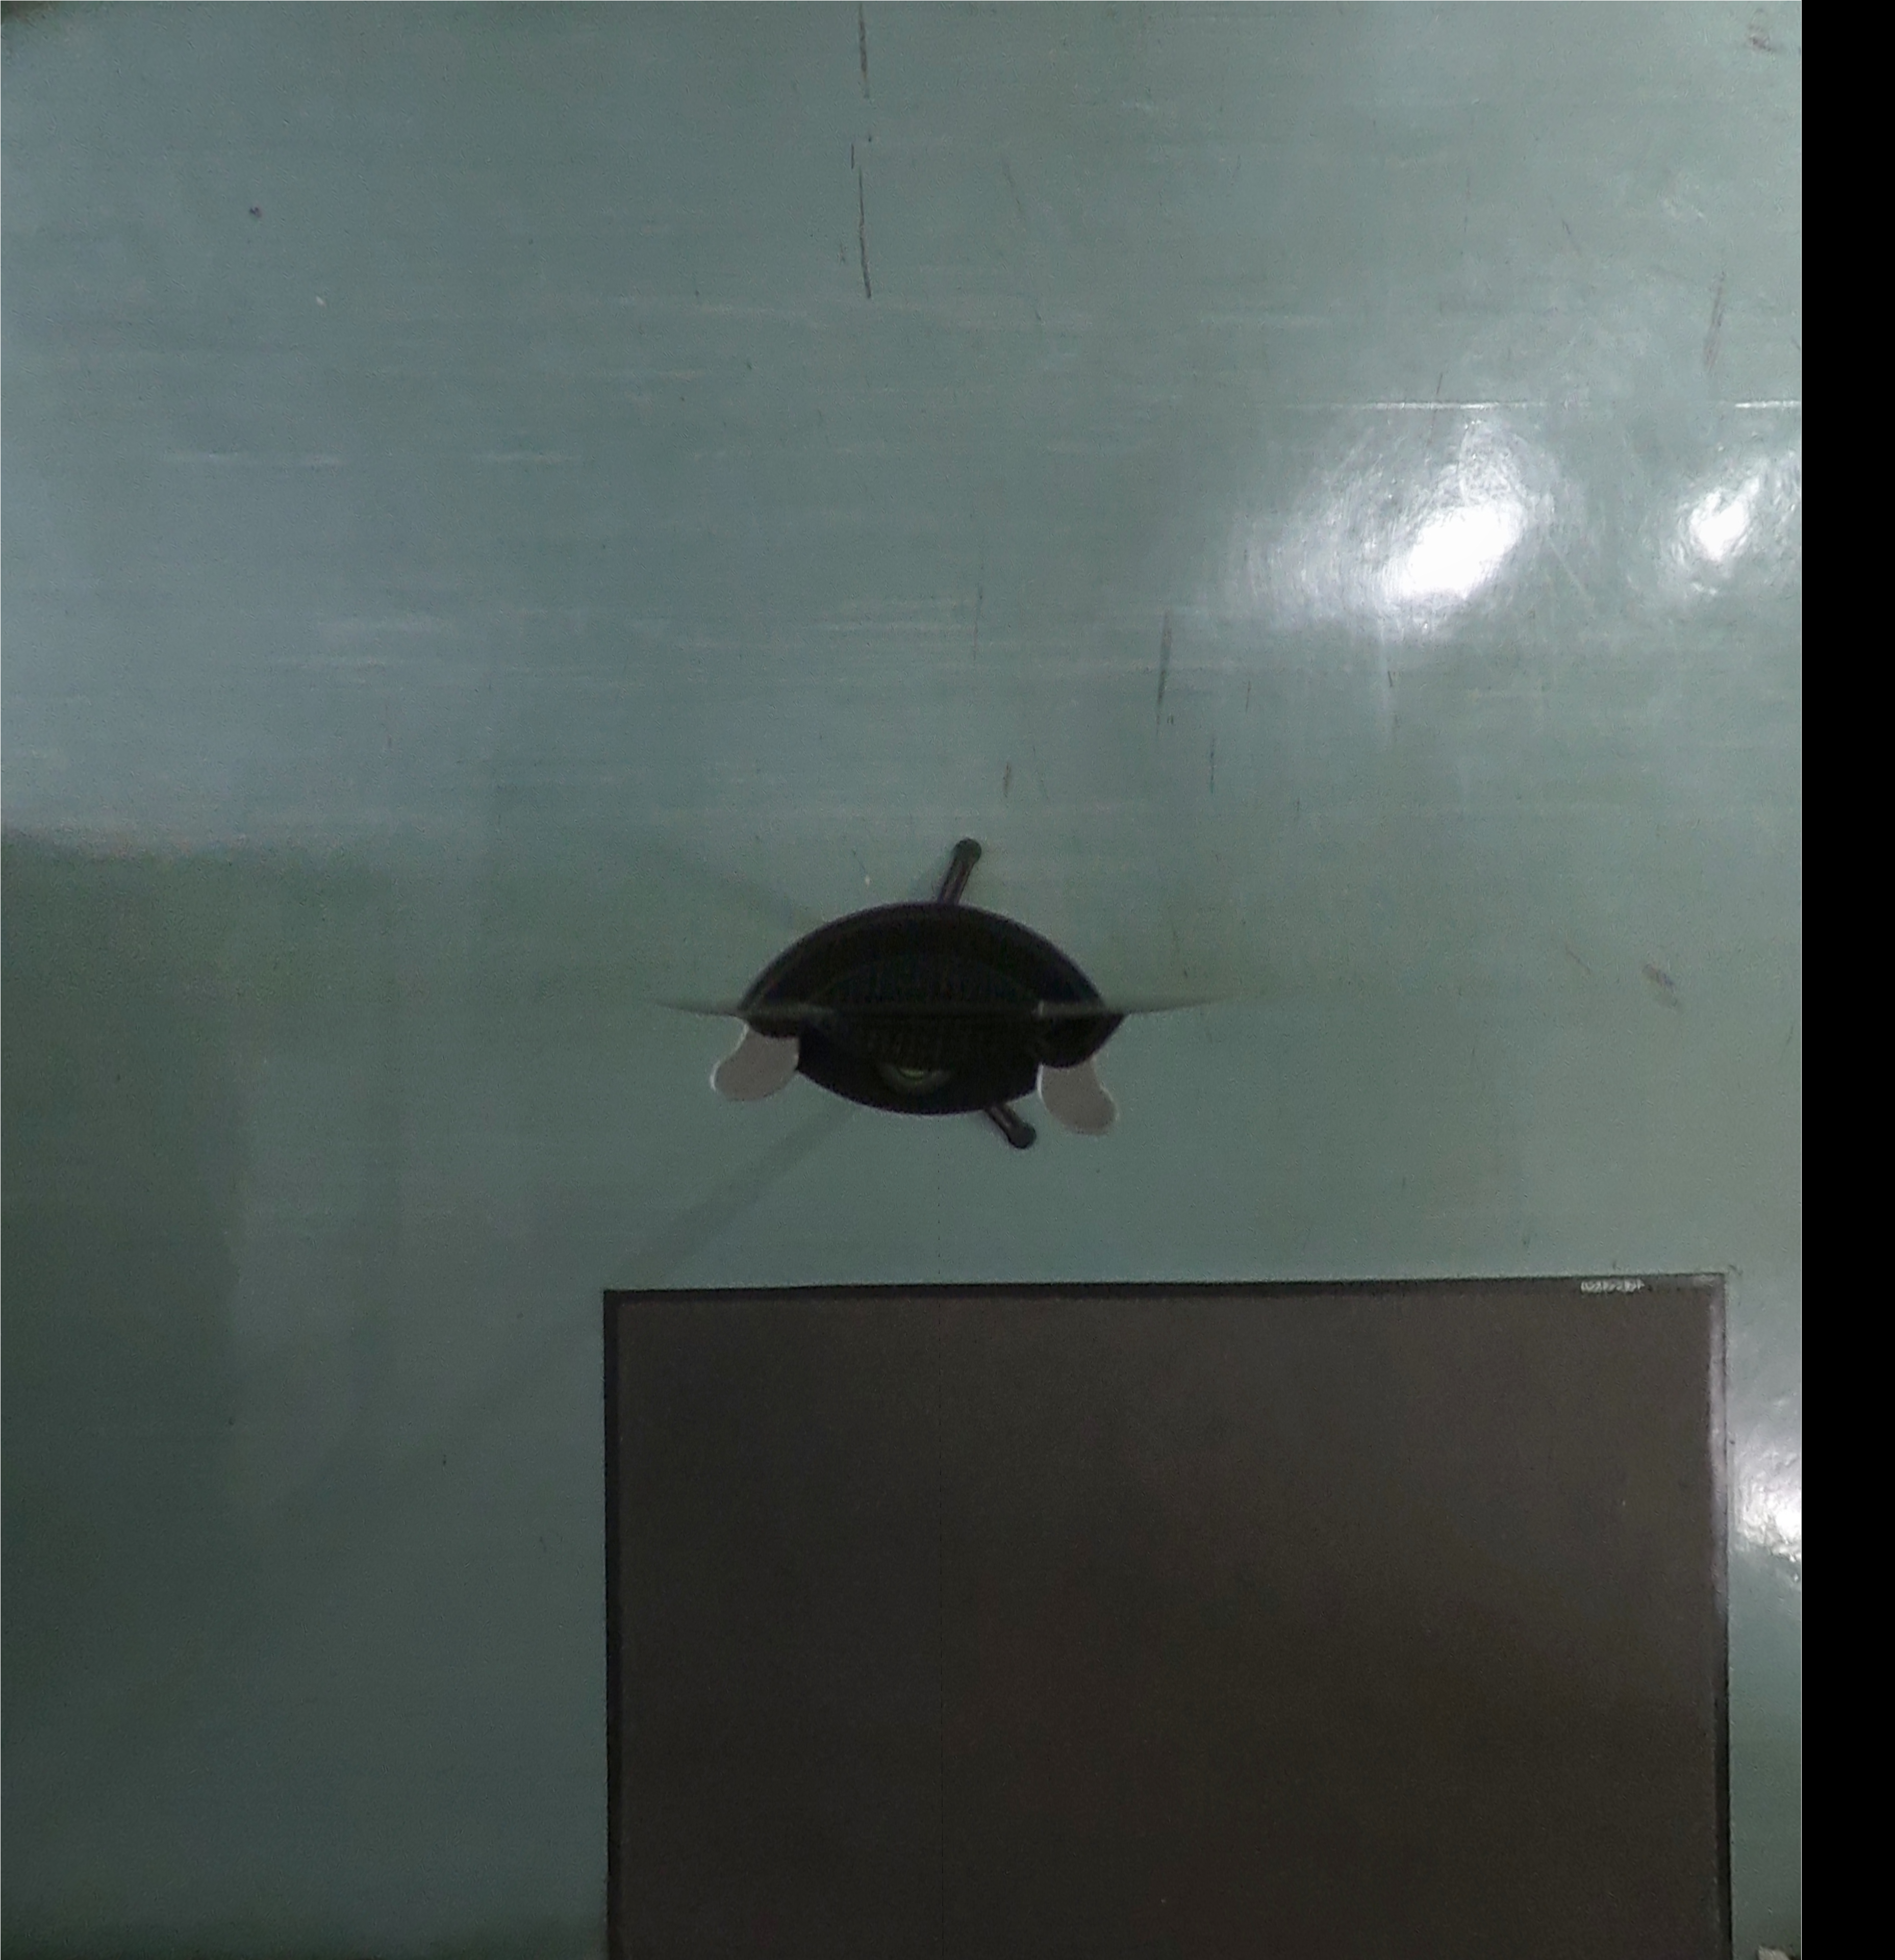
\includegraphics[keepaspectratio, scale=0.08]{figures/texture0/texture_0_0.png}&
      \includegraphics[keepaspectratio, scale=0.08]{figures/texture0/texture_0_5.png}\\
      \includegraphics[keepaspectratio, scale=0.08]{figures/texture0/texture_0_10.png}&
      \includegraphics[keepaspectratio, scale=0.08]{figures/texture0/texture_0_15.png}\\
    \end{tabular}
  \end{center}
  \caption{テクスチャ画像(全方位カメラ1)}
  \label{two}
\end{figure}

これらを用いて生成された3次元モデルを\hyperref[three]{図\ref{three}}に示す。

\begin{figure}[H]
  \begin{center}
    \begin{tabular}{c}
      \includegraphics[keepaspectratio, scale=0.4]{figures/3dmodel0.png}
    \end{tabular}
  \end{center}
  \caption{3次元モデル(全方位カメラ1)}
  \label{three}
\end{figure}

\subsection{全方位カメラ2(緑)}
全方位カメラ2の全方位画像から取得したテクスチャの一部を\hyperref[four]{図\ref{four}}に示す。
\begin{figure}[H]
  \begin{center}
    \begin{tabular}{cc}
      \includegraphics[keepaspectratio, scale=0.08]{figures/texture1/texture_1_0.png}&
      \includegraphics[keepaspectratio, scale=0.08]{figures/texture1/texture_1_5.png}\\
      \includegraphics[keepaspectratio, scale=0.08]{figures/texture1/texture_1_10.png}&
      \includegraphics[keepaspectratio, scale=0.08]{figures/texture1/texture_1_15.png}\\
    \end{tabular}
  \end{center}
  \caption{テクスチャ画像(全方位カメラ2)}
  \label{four}
\end{figure}

これらを用いて生成された3次元モデルを\hyperref[five]{図\ref{five}}に示す。

\begin{figure}[H]
  \begin{center}
    \begin{tabular}{c}
      \includegraphics[keepaspectratio, scale=0.4]{figures/3dmodel1.png}
    \end{tabular}
  \end{center}
  \caption{3次元モデル(全方位カメラ2)}
  \label{five}
\end{figure}


\subsection{全方位カメラ3(赤)}
全方位カメラ3の全方位画像から取得したテクスチャの一部を\hyperref[six]{図\ref{six}}に示す。
\begin{figure}[H]
  \begin{center}
    \begin{tabular}{cc}
      \includegraphics[keepaspectratio, scale=0.08]{figures/texture2/texture_2_0.png}&
      \includegraphics[keepaspectratio, scale=0.08]{figures/texture2/texture_2_5.png}\\
      \includegraphics[keepaspectratio, scale=0.08]{figures/texture2/texture_2_10.png}&
      \includegraphics[keepaspectratio, scale=0.08]{figures/texture2/texture_2_15.png}\\
    \end{tabular}
  \end{center}
  \caption{テクスチャ画像(全方位カメラ3)}
  \label{six}
\end{figure}

これらを用いて生成された3次元モデルを\hyperref[seven]{図\ref{seven}}に示す。

\begin{figure}[H]
  \begin{center}
    \begin{tabular}{c}
      \includegraphics[keepaspectratio, scale=0.4]{figures/3dmodel2.png}
    \end{tabular}
  \end{center}
  \caption{3次元モデル(全方位カメラ3)}
  \label{seven}
\end{figure}

\subsection{複数のカメラを用いた場合のテクスチャ及び全方位画像}
3つの全方位カメラの全方位画像から取得したテクスチャの一部を\hyperref[eight]{図\ref{eight}}に示す。
なお、複数のカメラで同一領域のテクスチャを取得した場合、重心の距離がカメラ中心に近いテクスチャを優先している。
そのため、実際に選択されるのは右側の2つのテクスチャである。

\begin{figure}[H]
  \begin{center}
    \begin{tabular}{cc}
      \includegraphics[keepaspectratio, scale=0.08]{figures/texture012/texture_0_13.png}&
      \includegraphics[keepaspectratio, scale=0.08]{figures/texture012/texture_2_10.png}\\
      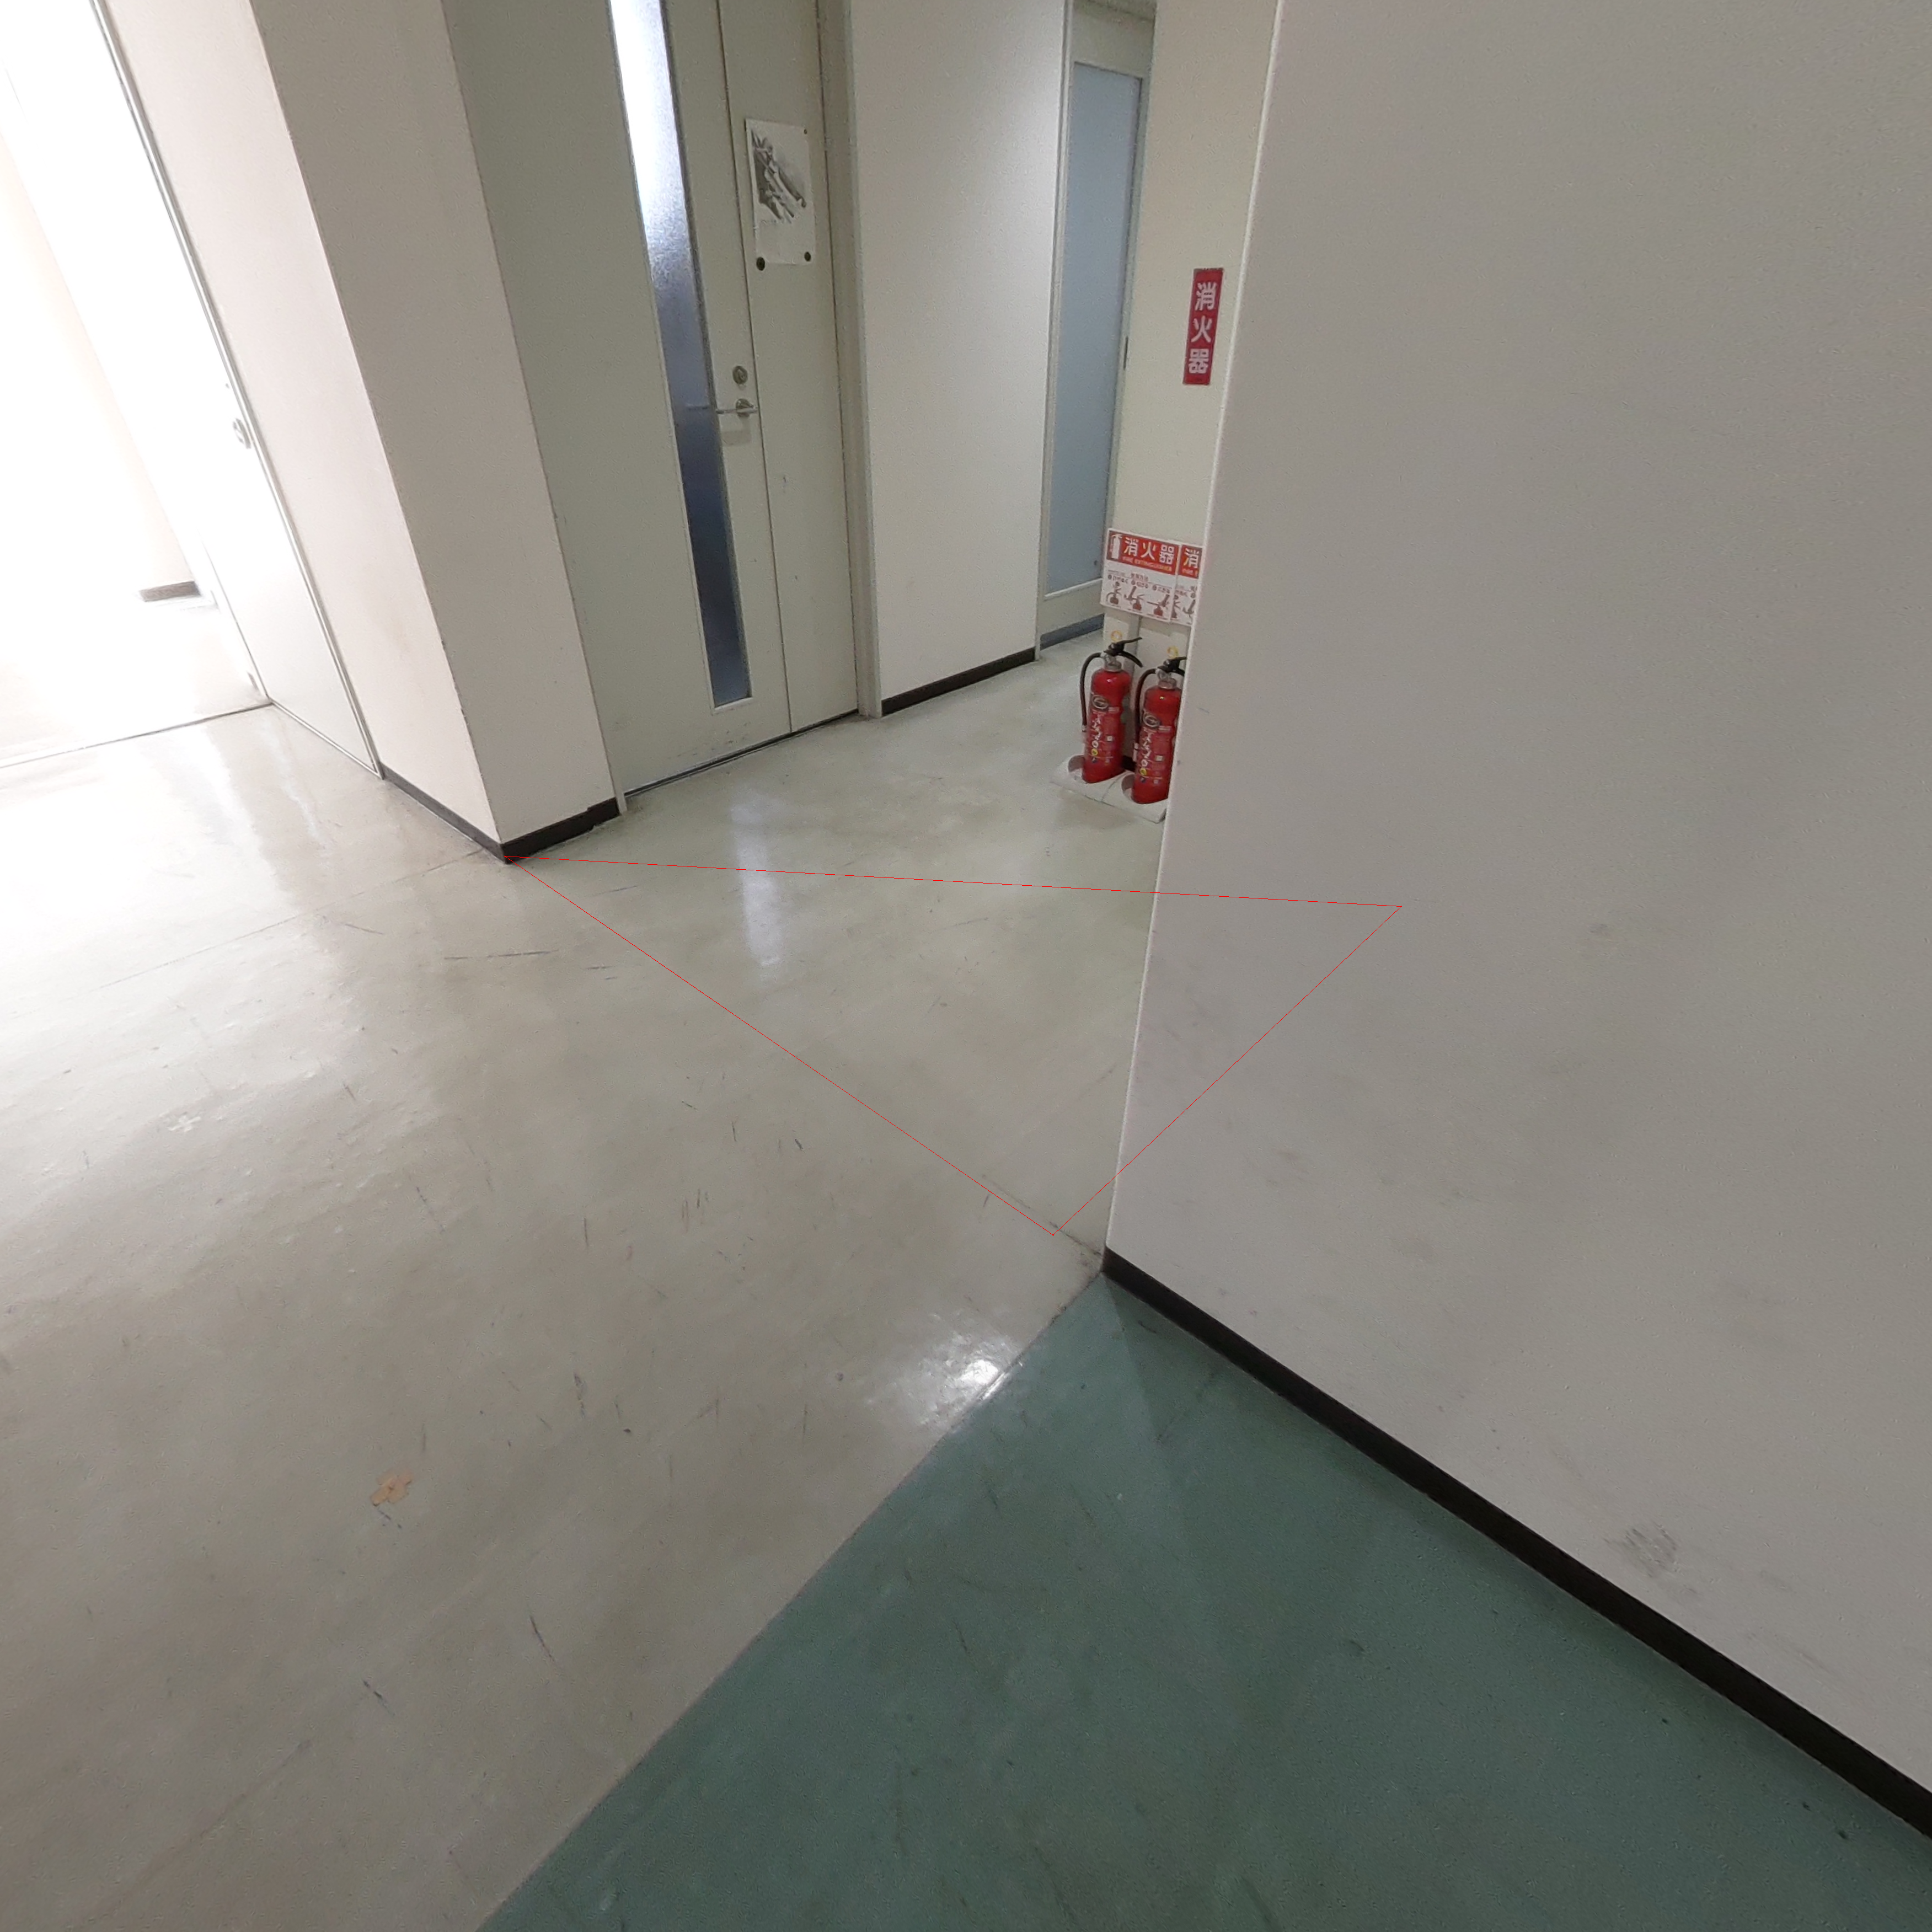
\includegraphics[keepaspectratio, scale=0.08]{figures/texture012/texture_2_12.png}&
      \includegraphics[keepaspectratio, scale=0.08]{figures/texture012/texture_1_17.png}\\
      \includegraphics[keepaspectratio, scale=0.08]{figures/texture012/texture_0_7.png}&
      \includegraphics[keepaspectratio, scale=0.08]{figures/texture012/texture_1_10.png}\\
      \includegraphics[keepaspectratio, scale=0.08]{figures/texture012/texture_1_3.png}&
      \includegraphics[keepaspectratio, scale=0.08]{figures/texture012/texture_2_1.png}\\
    \end{tabular}
  \end{center}
  \caption{テクスチャ画像(すべての全方位カメラ)}
  \label{eight}
\end{figure}

これらを用いて生成された3次元モデルを\hyperref[nine]{図\ref{nine}}に示す。
すべての面のテクスチャを取得することができているが、異なる全方位画像を用いている部分では明るさが異なり、
またテクスチャのずれが発生している。

\begin{figure}[H]
  \begin{center}
    \begin{tabular}{c}
      \includegraphics[keepaspectratio, scale=0.4]{figures/3dmodel012.png}
    \end{tabular}
  \end{center}
  \caption{3次元モデル(すべての全方位カメラ)}
  \label{nine}
\end{figure}

\subsection{今後の目標}
プログラムの問題点については修正し、単一の全方位画像であればある程度3次元モデルを再現することができたが、
複数の全方位画像を結合するとずれが発生してしまった。
この要因の一つとして全方位画像の撮影間隔が大きすぎることがあると考える。
しかし、現時点では2次元座標と3次元座標の対応付けを手動で行っているため、
撮影間隔を小さくして大量の全方位画像を用いると、対応付けがとても大変になってしまう。
そのため、この点を解決する方法を模索していく必要がある。
また明るさの調節なども含めて別の方法で3次元モデルの再現度を高めることについても検討する。
\end{document}
